%
% About the Authors
%

\section*{About the authors}

%
% Peter Rohde
%

\begin{center}
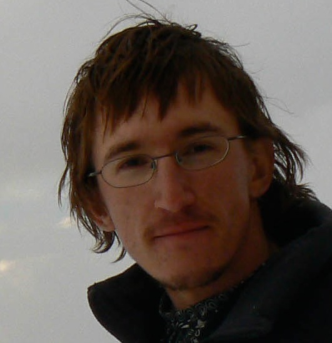
\includegraphics[width=0.47\textwidth]{photo_peter_rohde}
\end{center}

Peter Rohde is an ARC Future Fellow in the Centre for Quantum Software \& Information at the University of Technology Sydney, Australia (UTS:Q$|$SI$\rangle$), and associate member of the Hearne Institute for Theoretical Physics at Louisiana State University. He obtained a Bachelor of Computer Systems Engineering with First Class Honours, and a PhD in theoretical physics at the University of Queensland. He has worked at highly-acclaimed international institutes, including the University of Oxford, University of Queensland, Institute for Molecular Biosciences and Max-Planck Institute for the Science of Light, with over 50 publications and 1,300+ citations in quantum optics, quantum computing, quantum information theory and ecology. His theoretical proposals have inspired several world-leading experimental efforts, including time-bin encoded \textsc{BosonSampling} and sub-shot-noise limited quantum metrology. In his spare time he is a musician, composer, public speaker, charity worker, mountaineer and adrenaline junkie. He regularly speaks at prominent scientific outreach events, features in newspaper and magazine articles, and conducts radio interviews. He is a very naughty boy and was expelled from preschool.

%
% Heliang Huang
%

\begin{center}
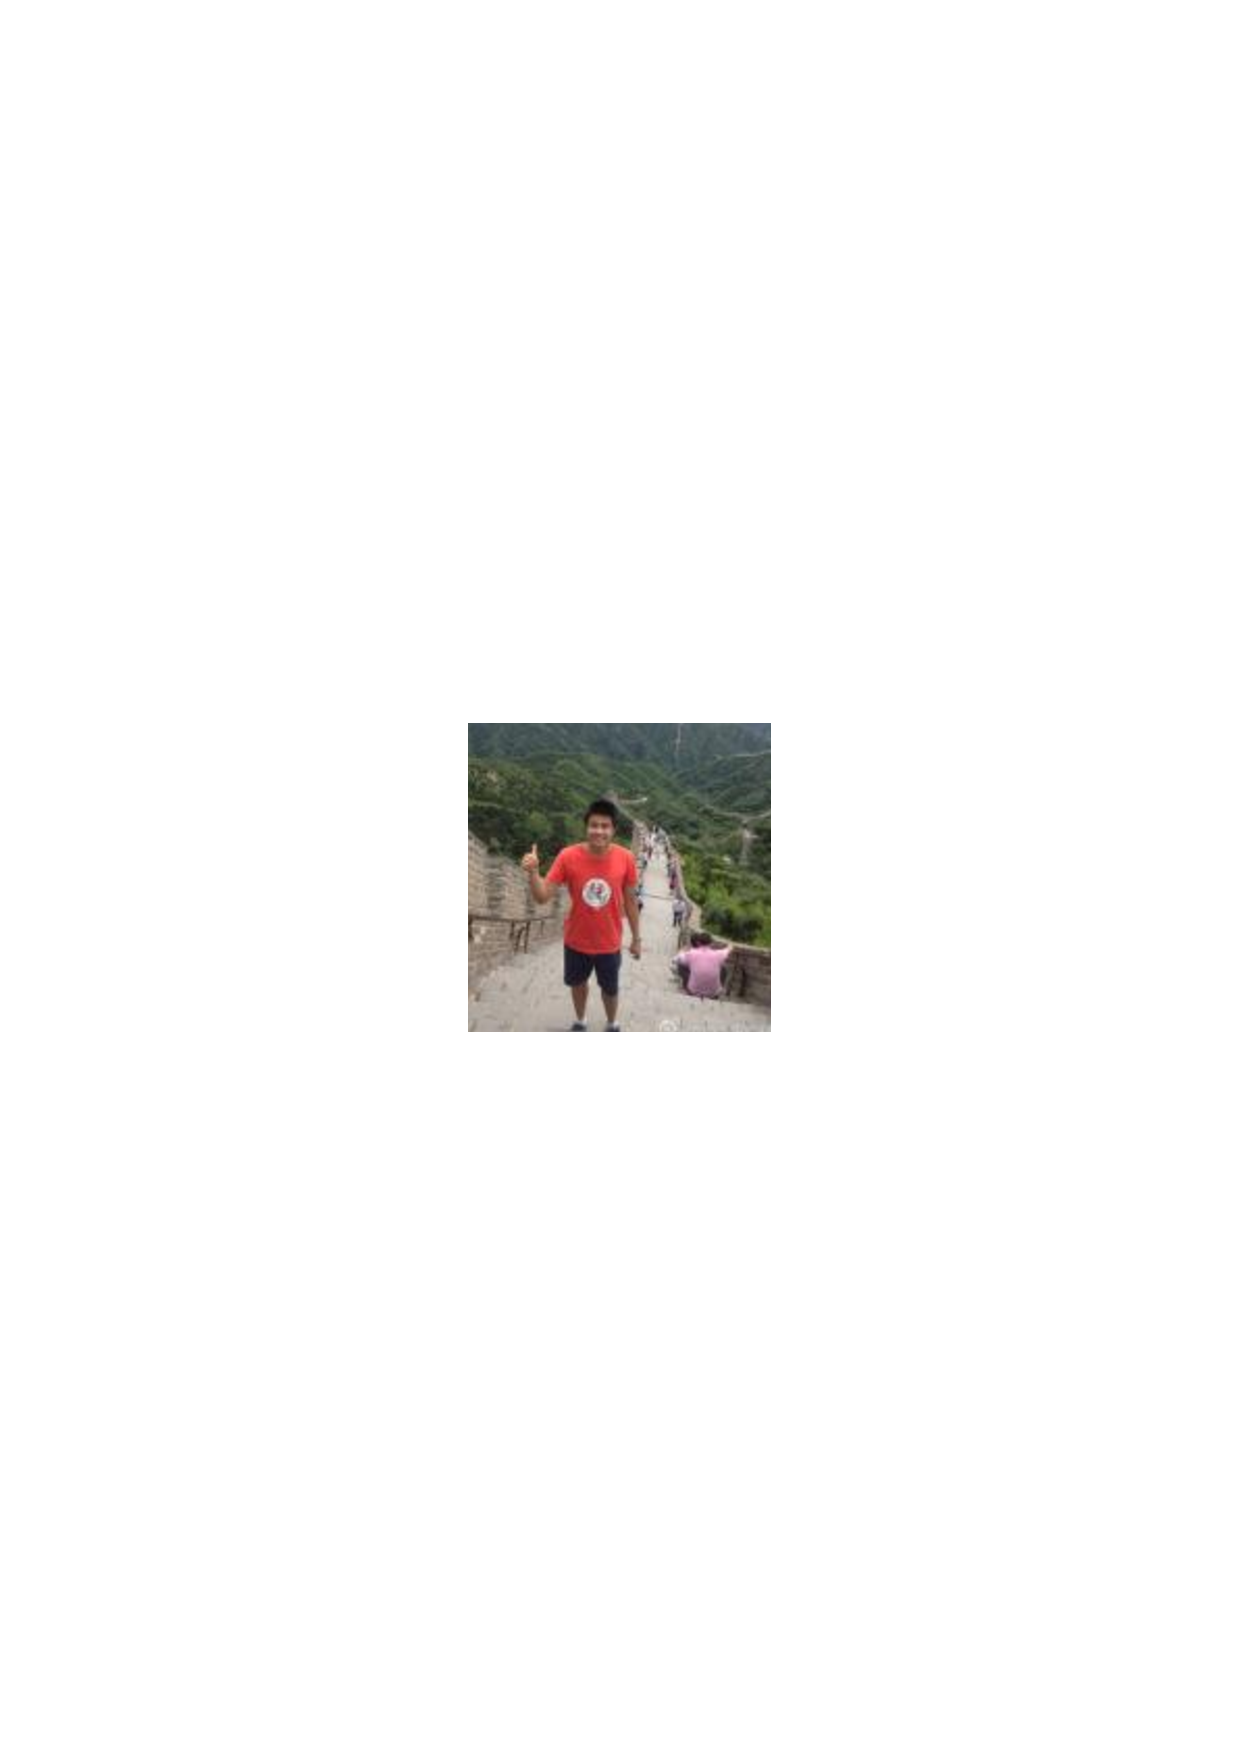
\includegraphics[width=0.47\textwidth]{photo_heliang_huang}
\end{center}

He-Liang Huang is a PhD candidate at the University of Science \& Technology China.x

%
% Zuen Su
%

\begin{center}

\includegraphics[width=0.47\textwidth]{photo_zuen_su}
\end{center}

Zu-En Su is a PhD candidate at the University of Science \& Technology China.

\comment{Complete this section}

%
% Zixin Huang
%

\begin{center}
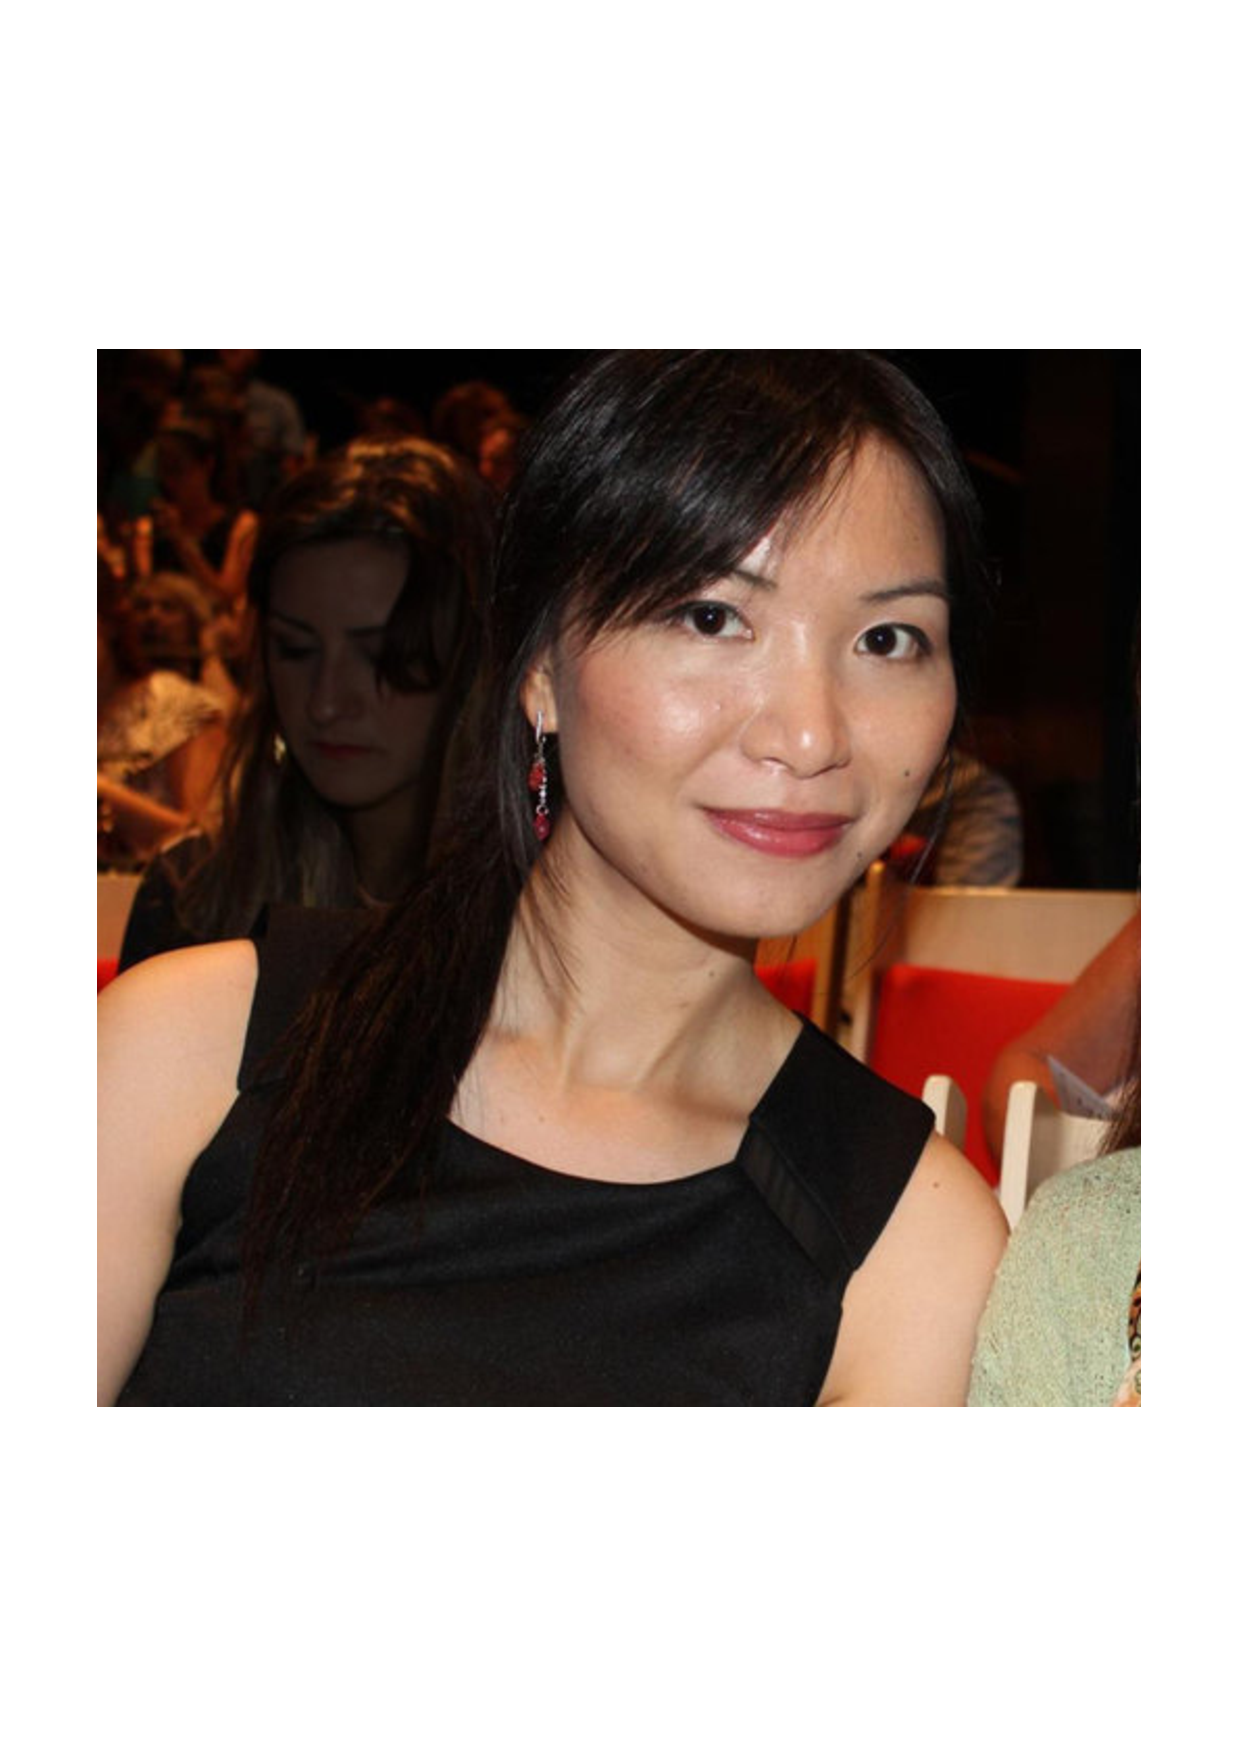
\includegraphics[width=0.47\textwidth]{photo_zixin_huang}
\end{center}

Zixin Huang completed her PhD in physics at the University of Sydney, Australia. She is currently a postdoctoral fellow at the University of Sheffield, UK.

\comment{Complete this section}

%
% Chris Ferrie
%

\begin{center}
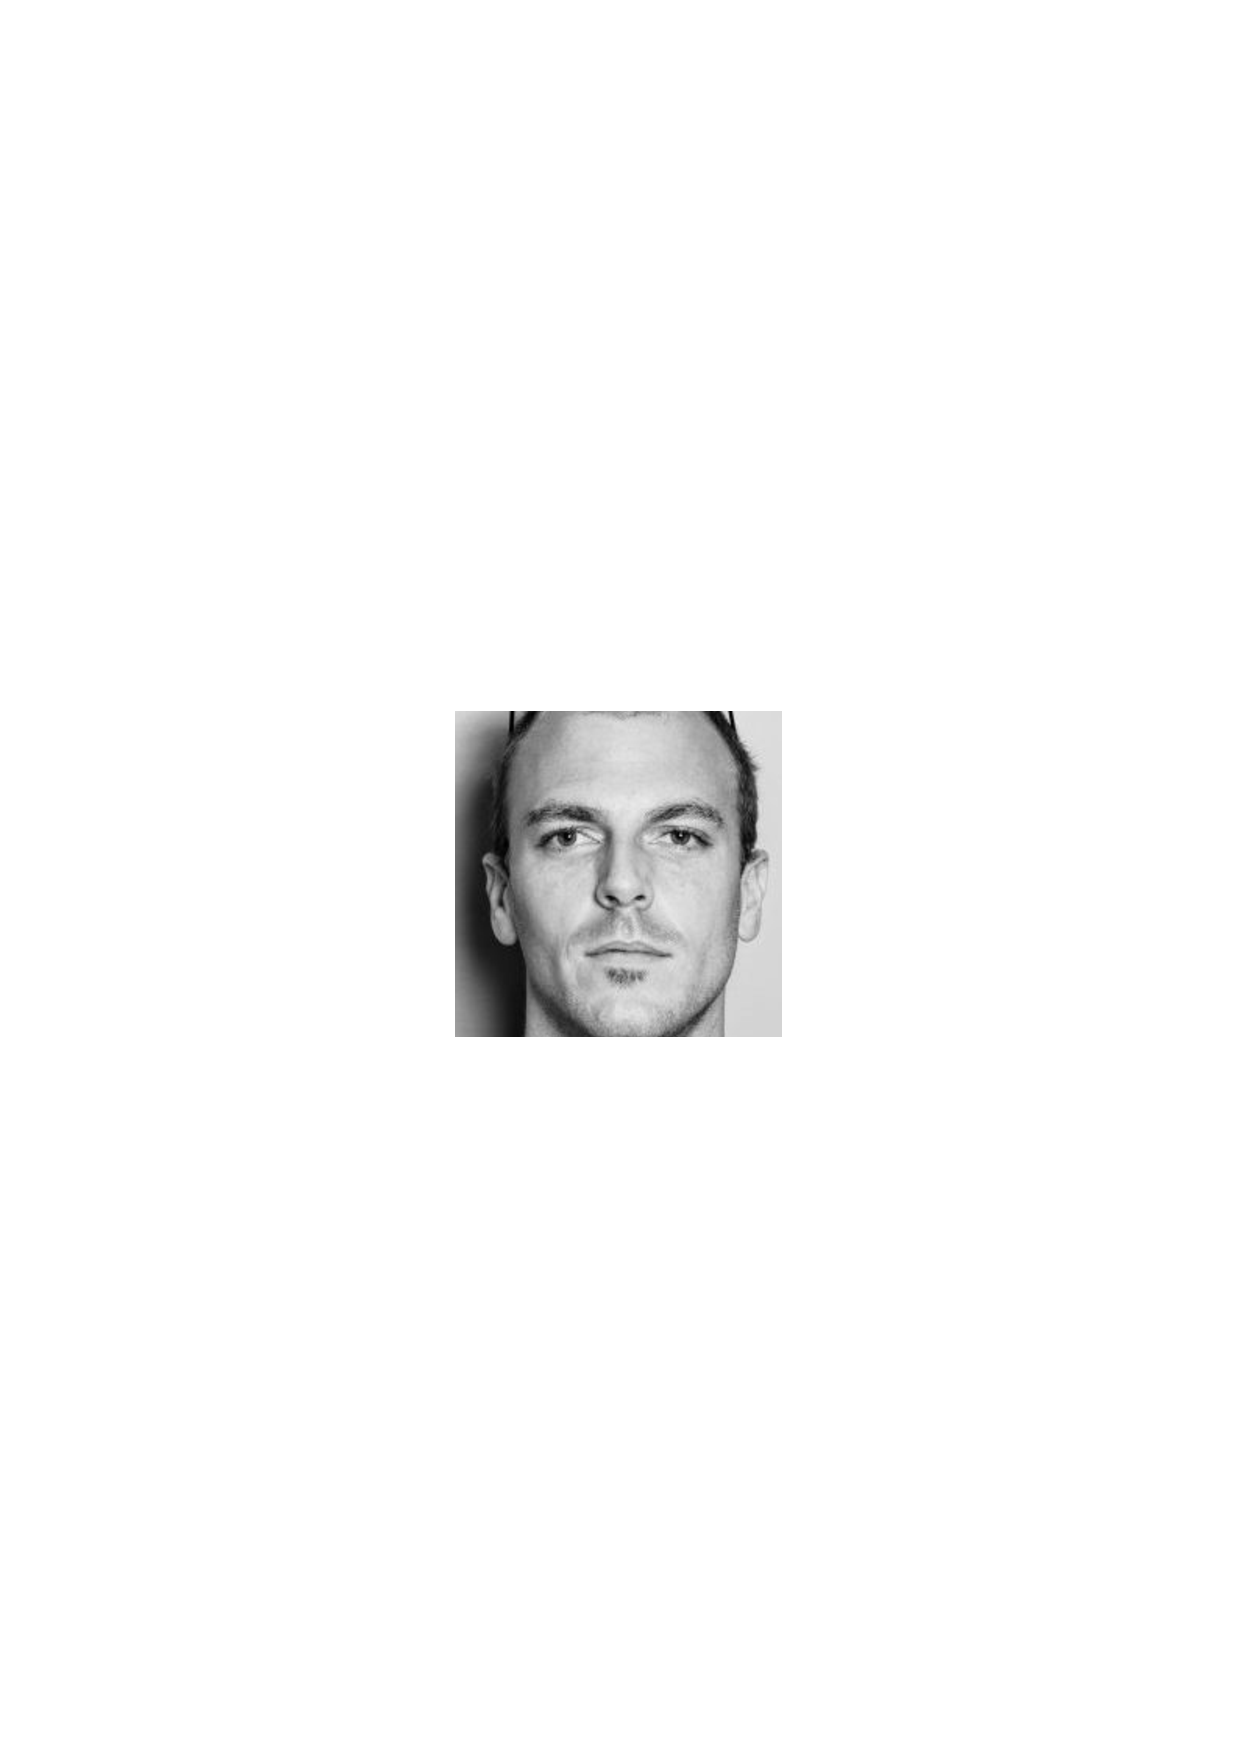
\includegraphics[width=0.47\textwidth]{photo_chris_ferrie}
\end{center}

\comment{Chris Ferrie}

%
% Simon Devitt
%

\begin{center}
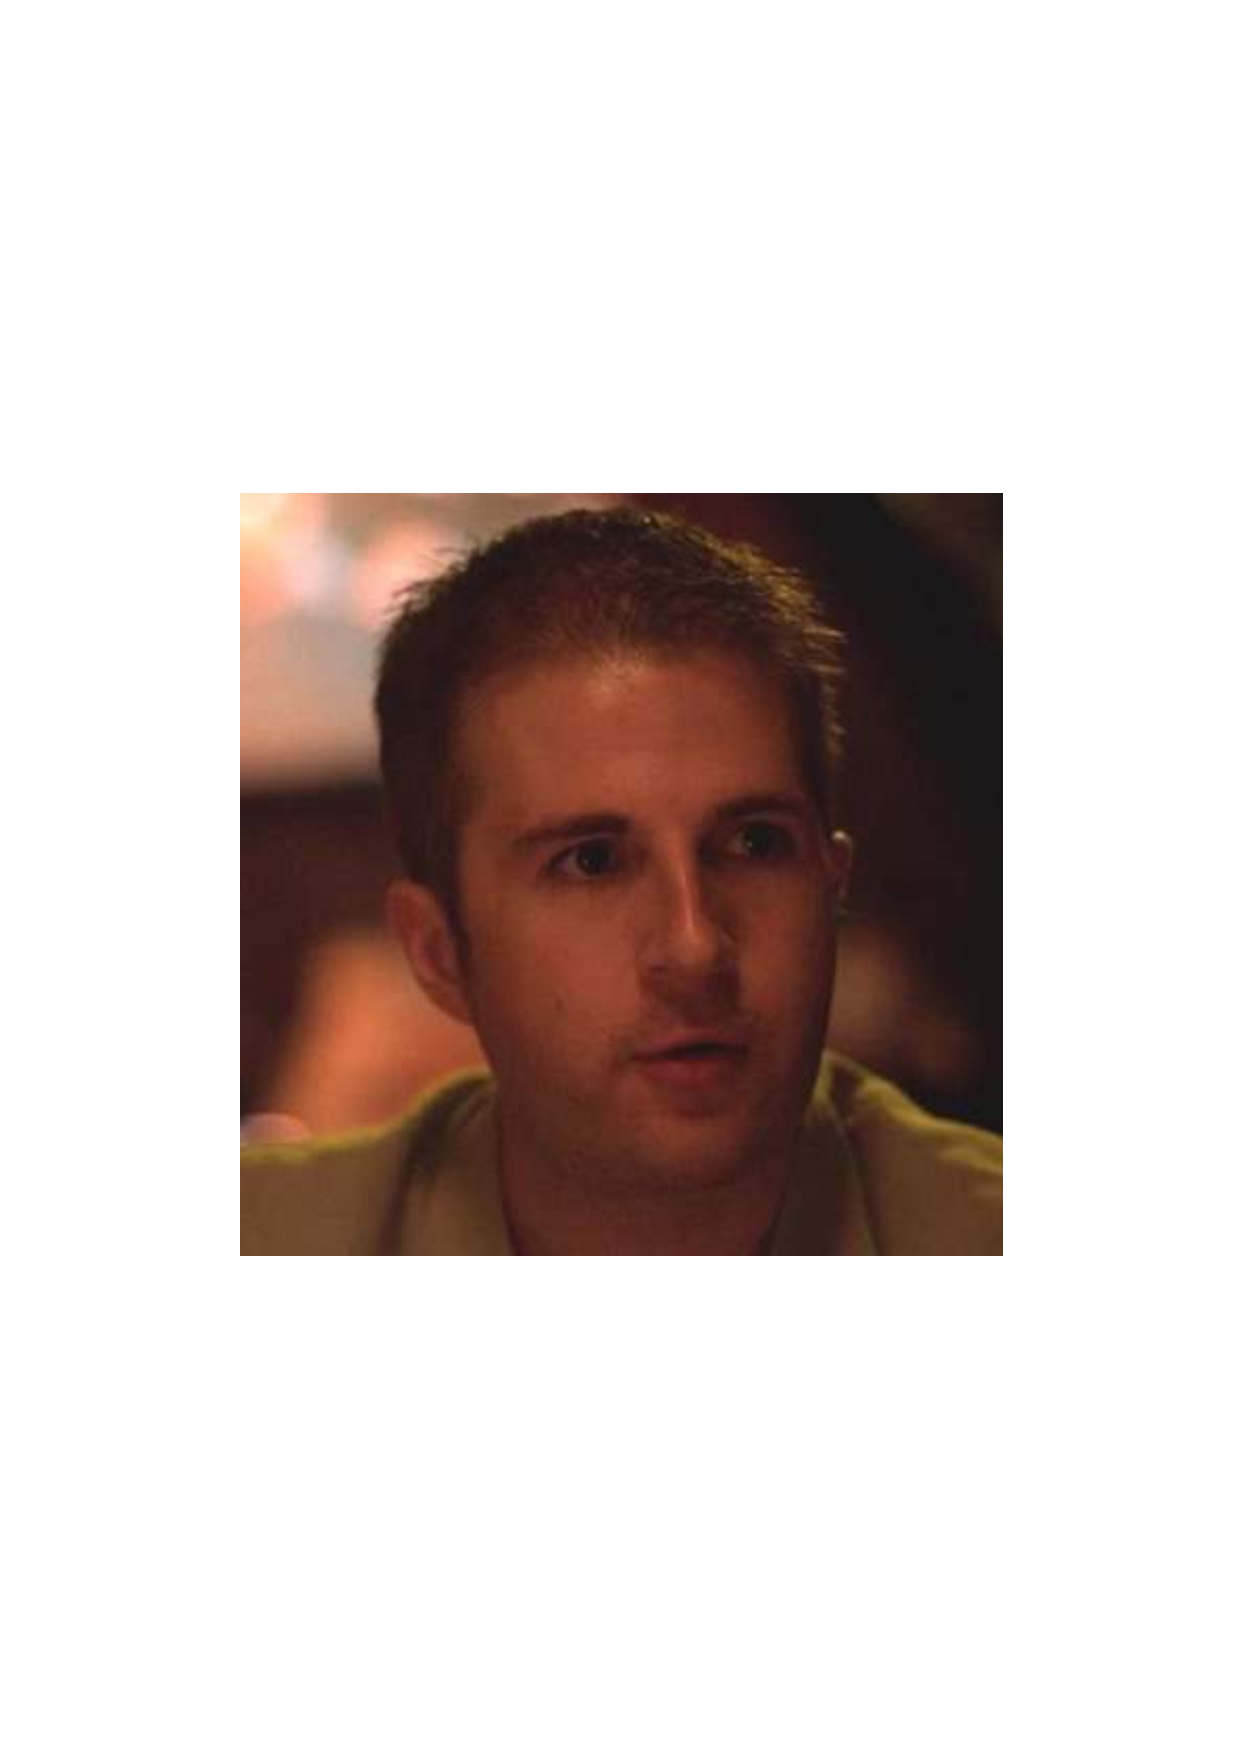
\includegraphics[width=0.47\textwidth]{photo_simon_devitt}
\end{center}

\comment{Simon Devitt}

%
% Si-Hui Tan
%

\begin{center}
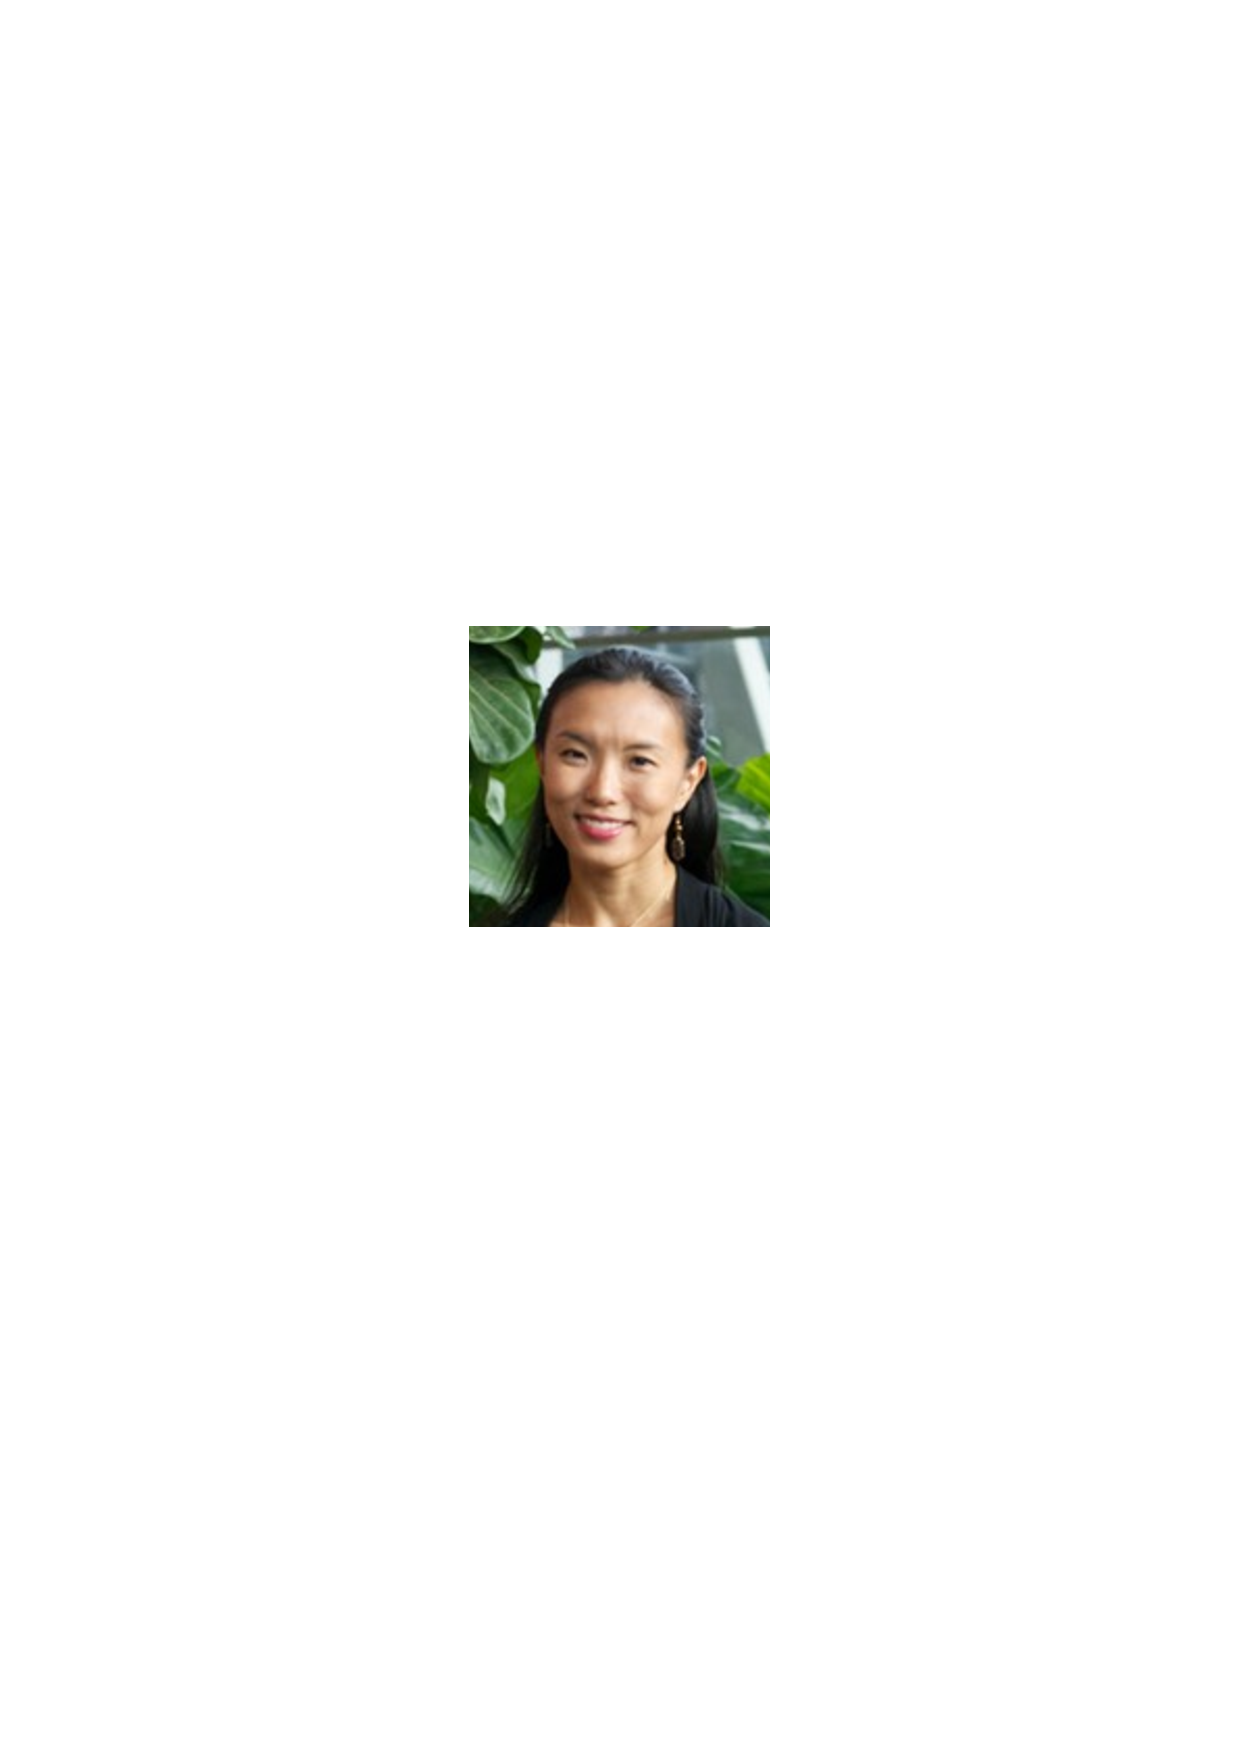
\includegraphics[width=0.47\textwidth]{photo_sihui_tan}
\end{center}

Si-Hui Tan is a Research Scientist at the Singapore University of Technology \& Design. She obtained a Bachelor of Science with Honours from Caltech, and subsequently a PhD from MIT. She has received numerous awards, including the MIT Presidential Fellowship.

\comment{Complete this section}

%
% Nana Liu
%

\begin{center}
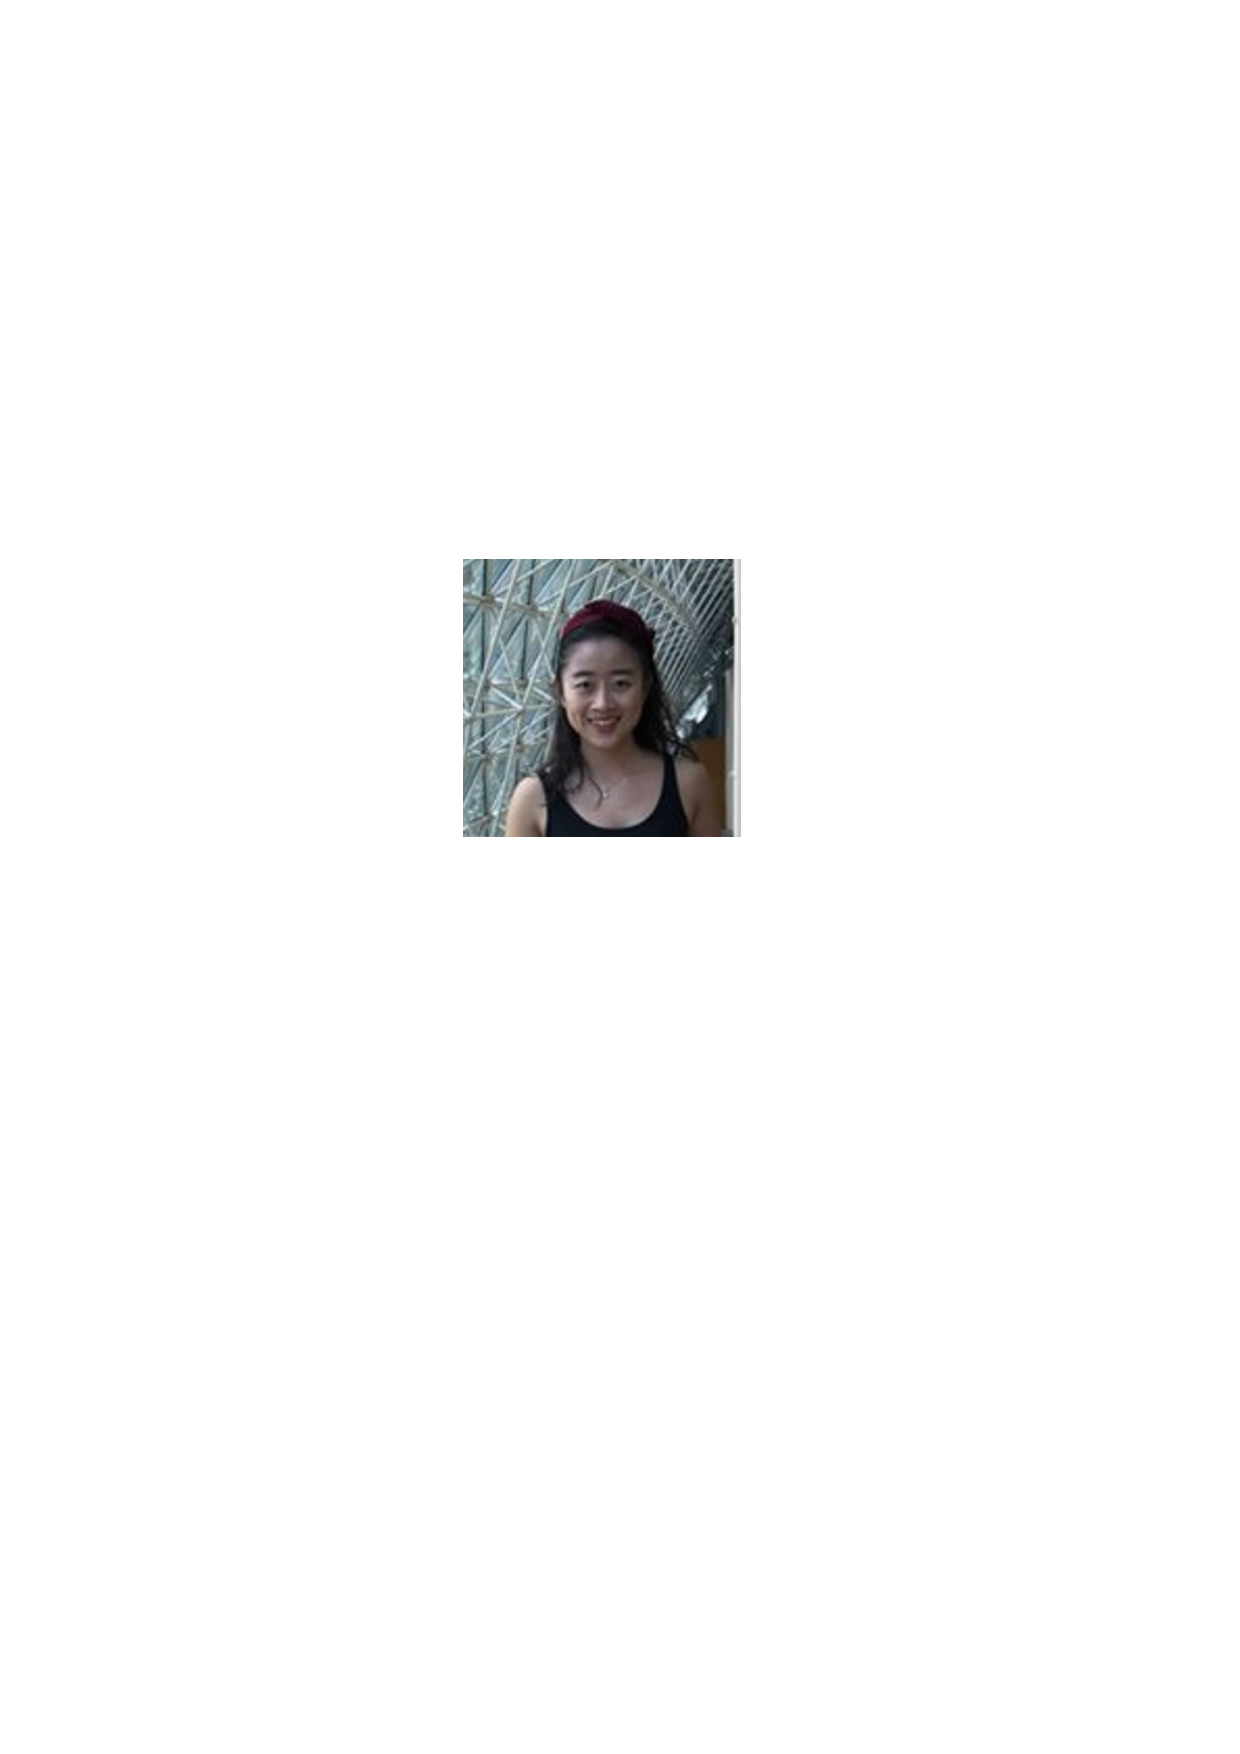
\includegraphics[width=0.47\textwidth]{photo_nana_liu}
\end{center}

Nana Liu is a Postdoctoral Research Fellow at the Singapore University of Technology \& Design.

\comment{Complete this section}

%
% Ryan Mann
%

%\begin{center}
%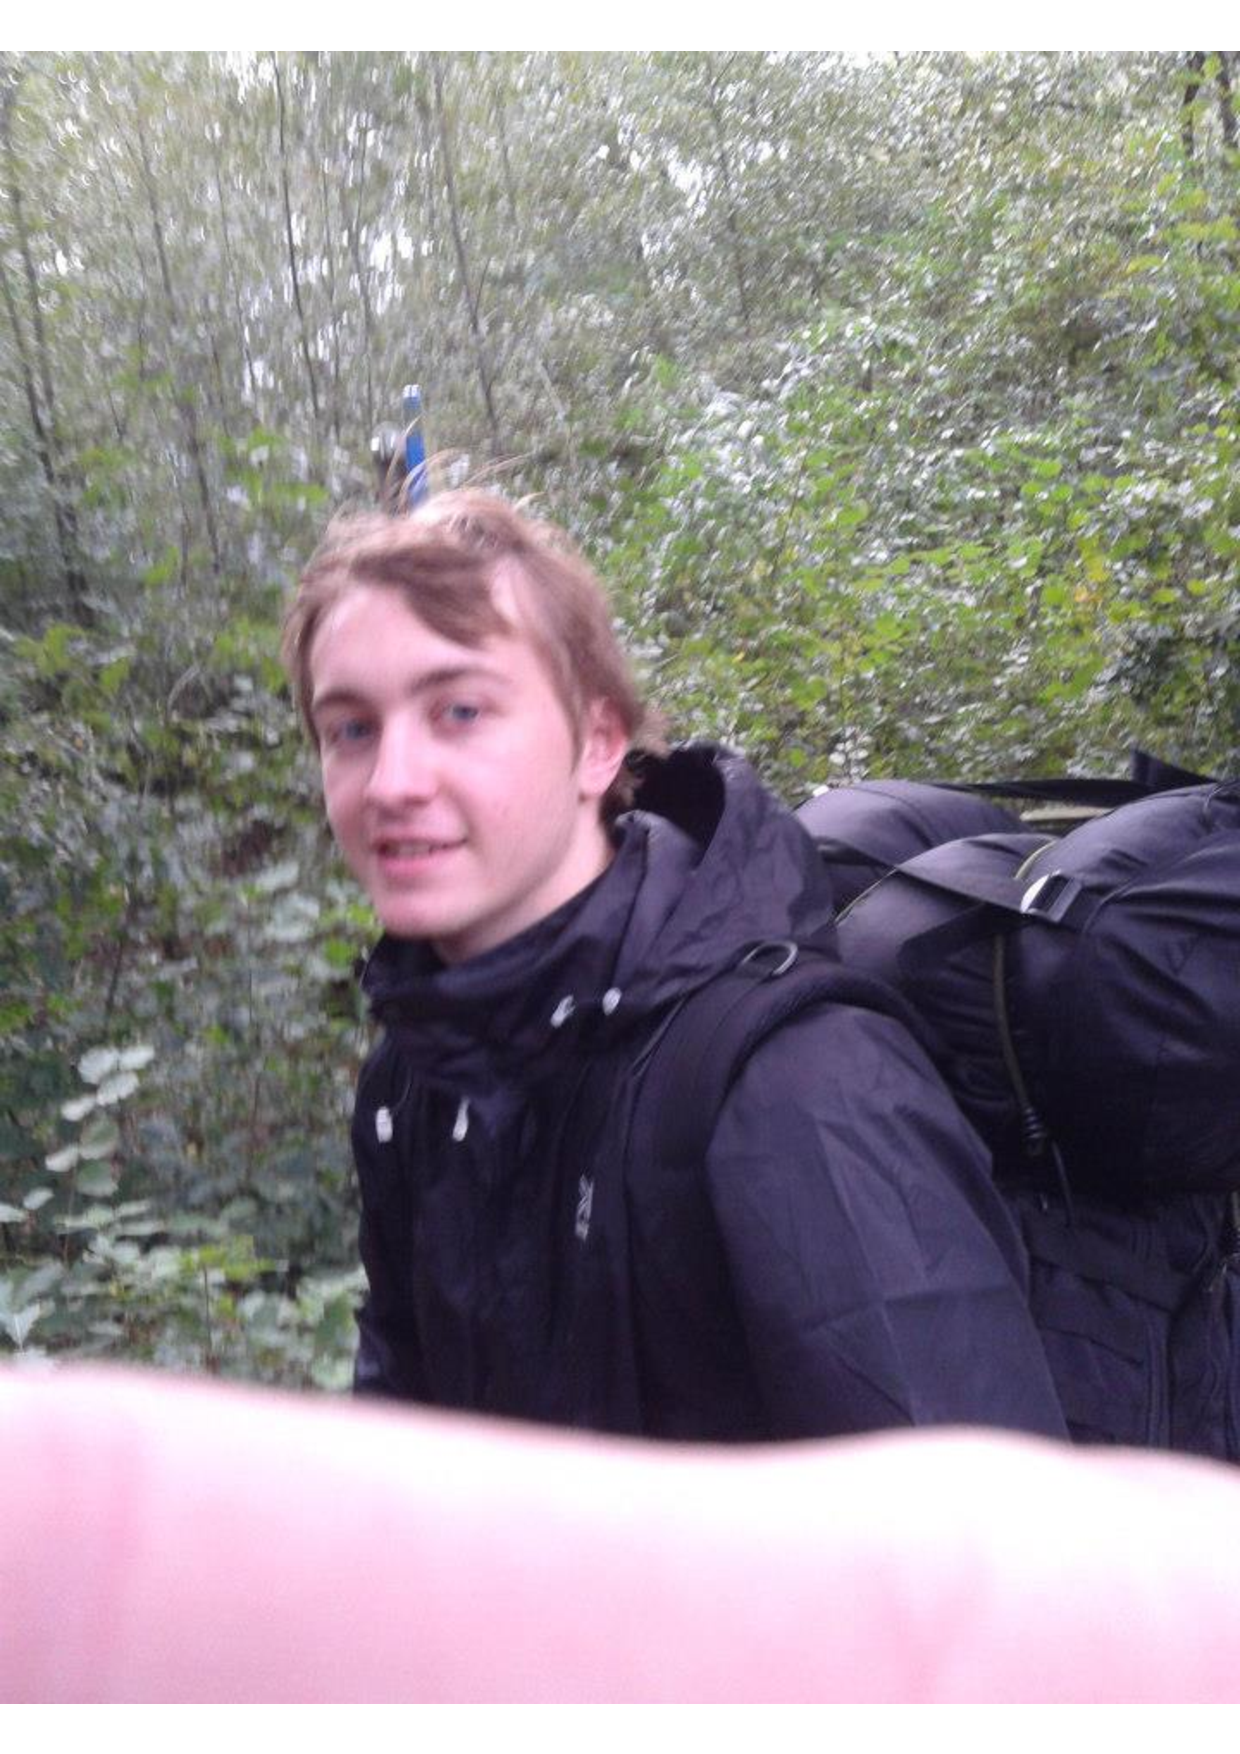
\includegraphics[width=0.47\textwidth]{photo_ryan_mann}
%\end{center}

%Ryan Mann is a PhD candidate in the Centre for Quantum Software \& Information at the University of Technology Sydney. He is a better rock-climber than he is physicist, despite being outstanding at the latter.

%\comment{Complete this section}

%
% Rohit Ramakrishnan
%

\begin{center}
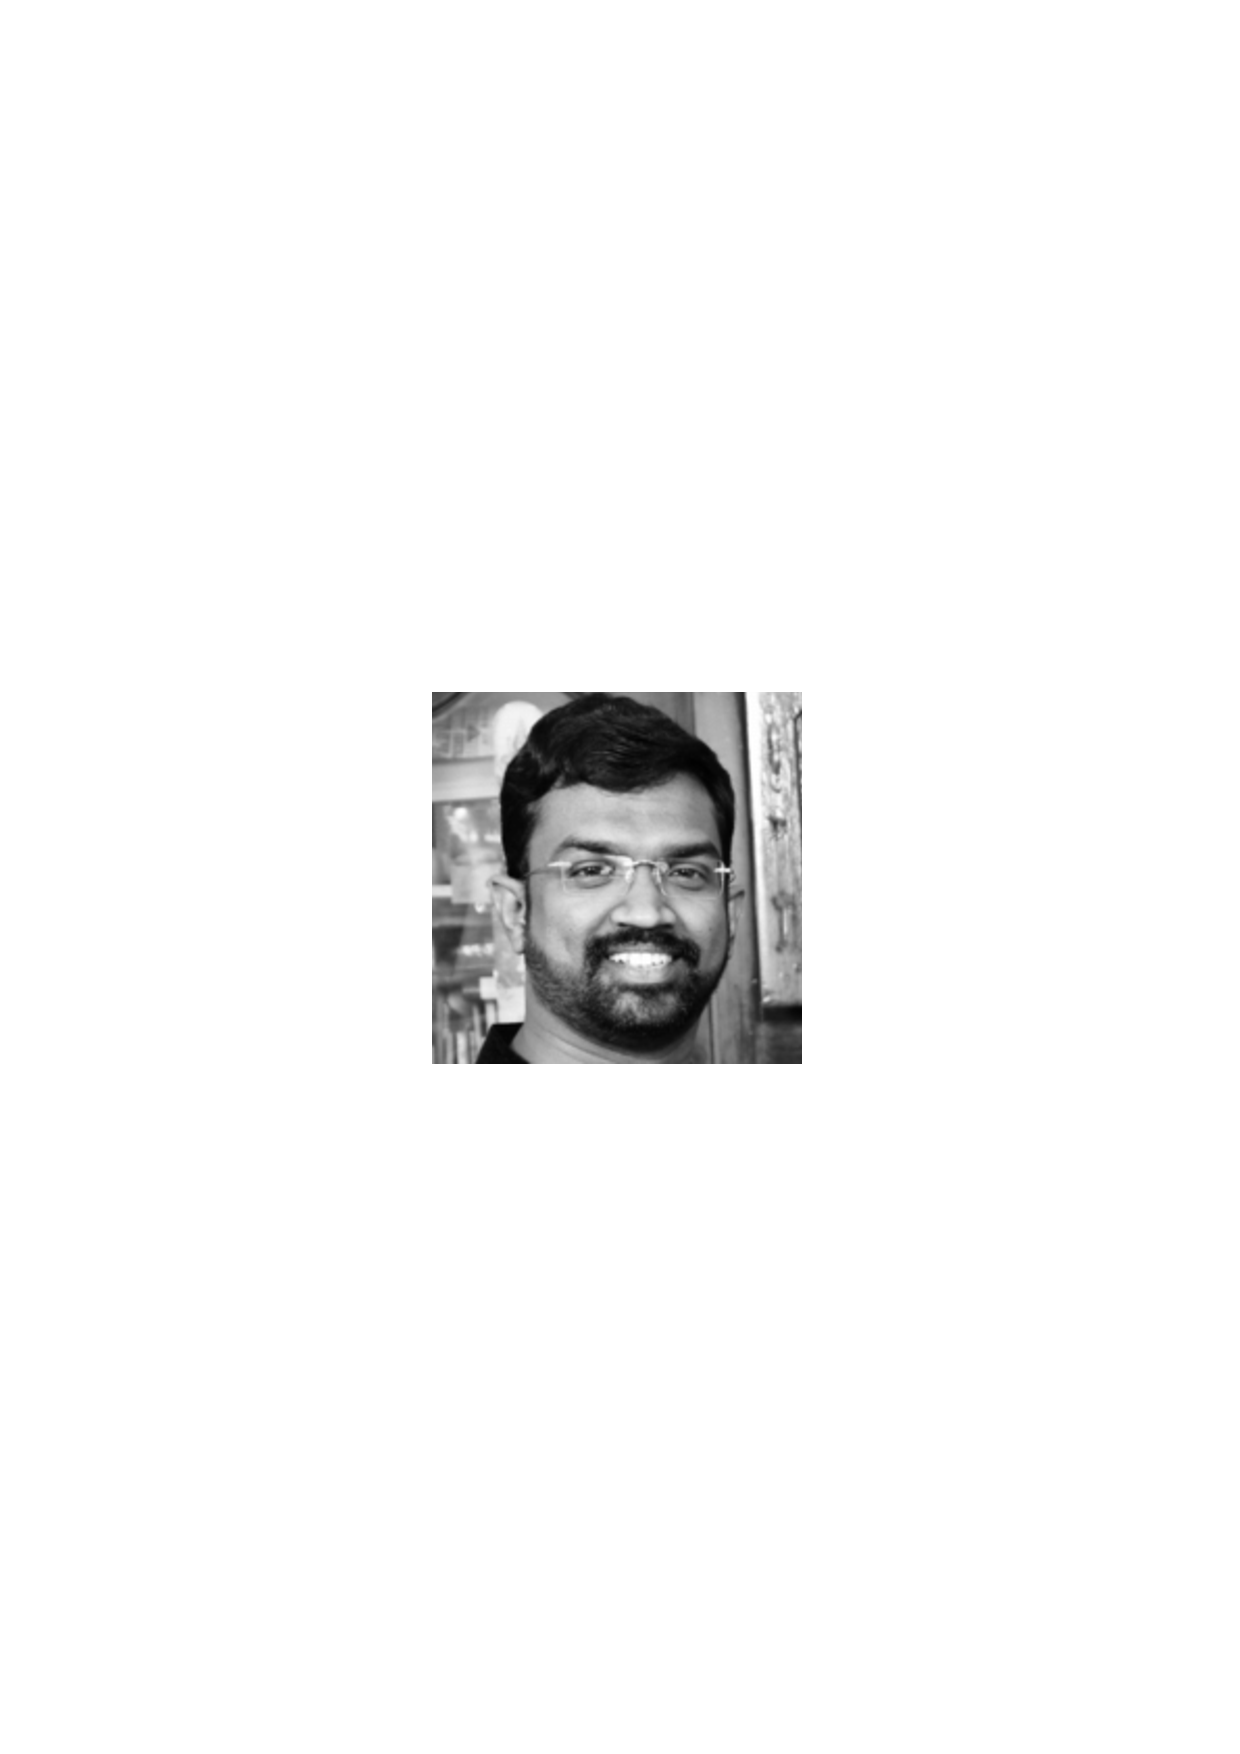
\includegraphics[width=0.47\textwidth]{photo_rohit_ramakrishnan}
\end{center}

Rohit Ramakrishnan is a researcher at the Indian Institute of Science.

\comment{Complete this section}

%
% Jon Dowling
%

\begin{center}
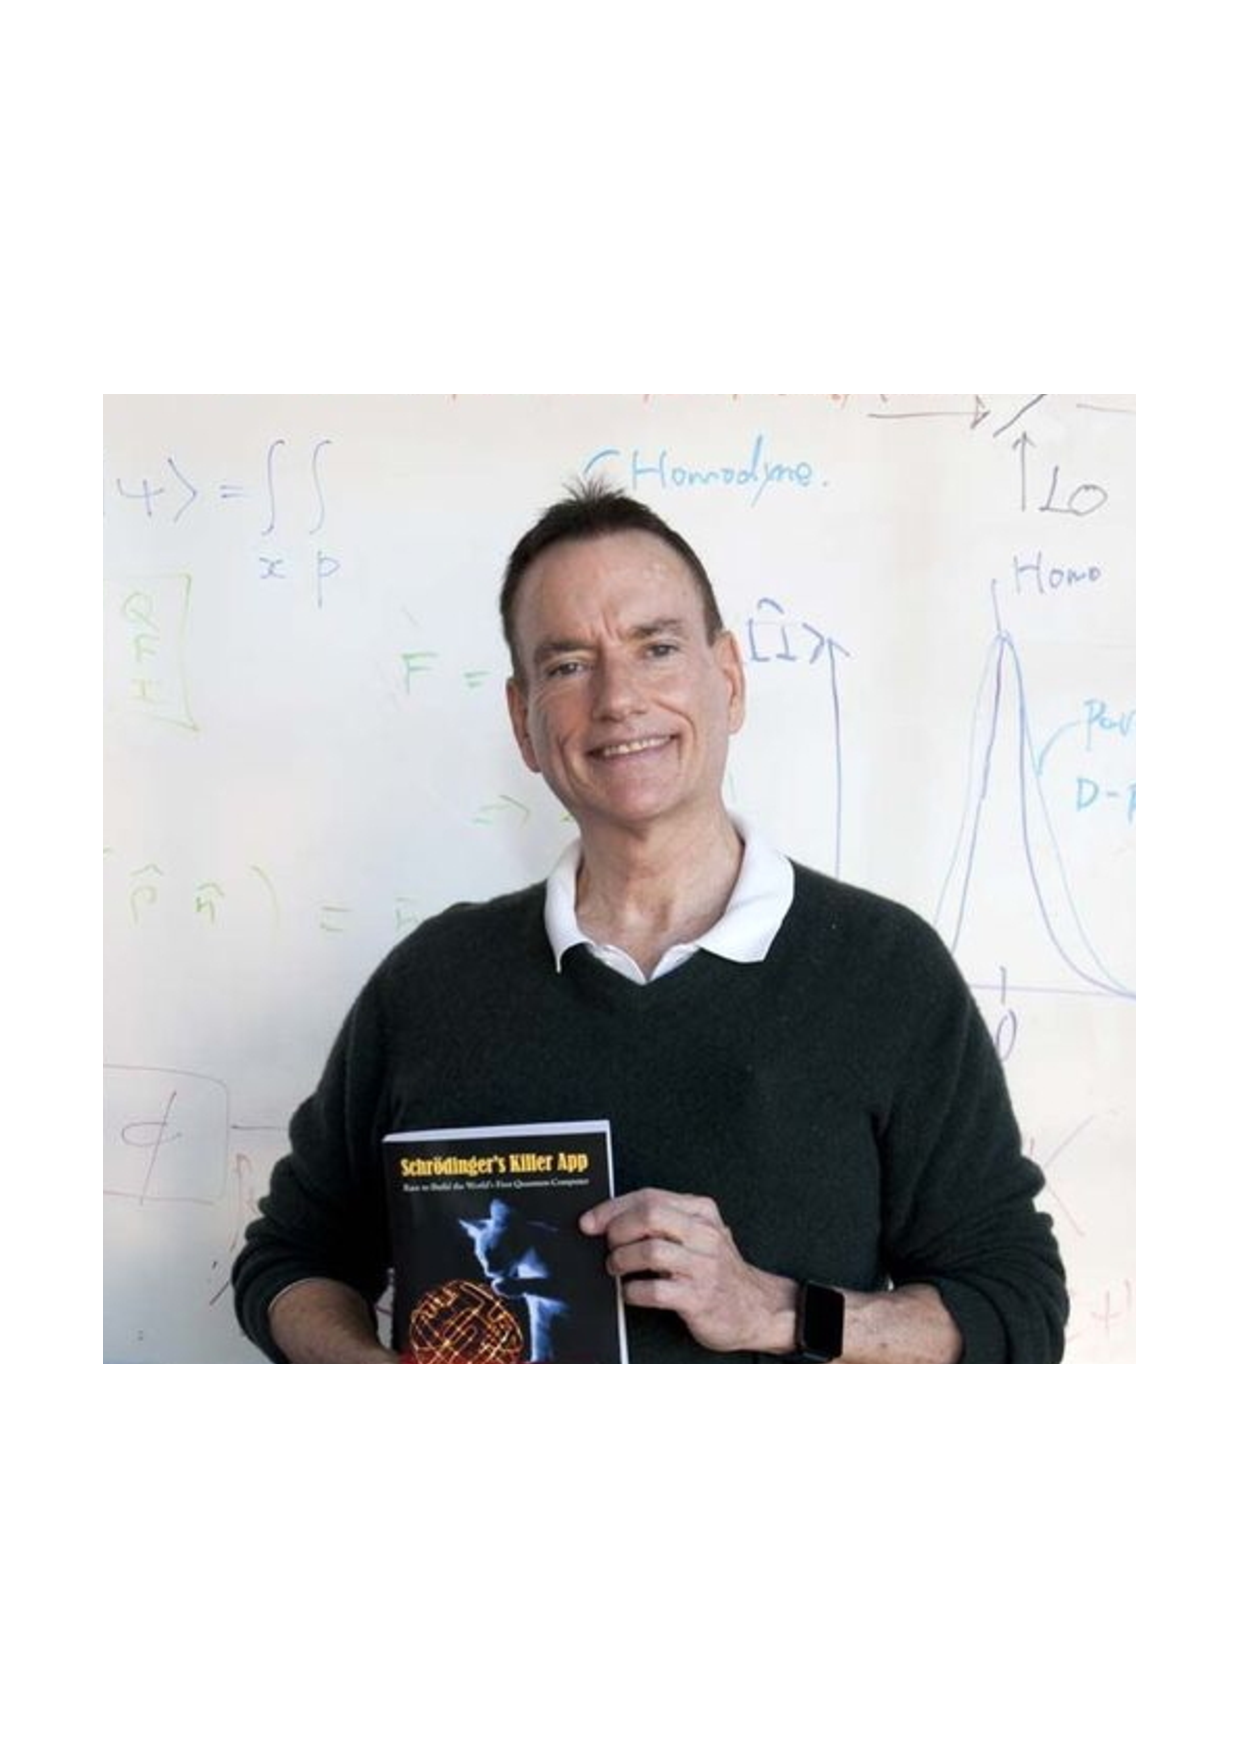
\includegraphics[width=0.47\textwidth]{photo_jon_dowling}
\end{center}

Jon Dowling is Professor and Hearne Chair of Theoretical Physics, and Co-Director of the Hearne Institute for Theoretical Physics at Louisiana State University. He has a highly-acclaimed research career, with over 450 publications and 15,000 citations. He is author of the popular book \textit{Schr\"odinger's Killer App: Race to Build the World's First Quantum Computer}.

\comment{Complete this section}

%
% Tim Byrnes
%

\begin{center}
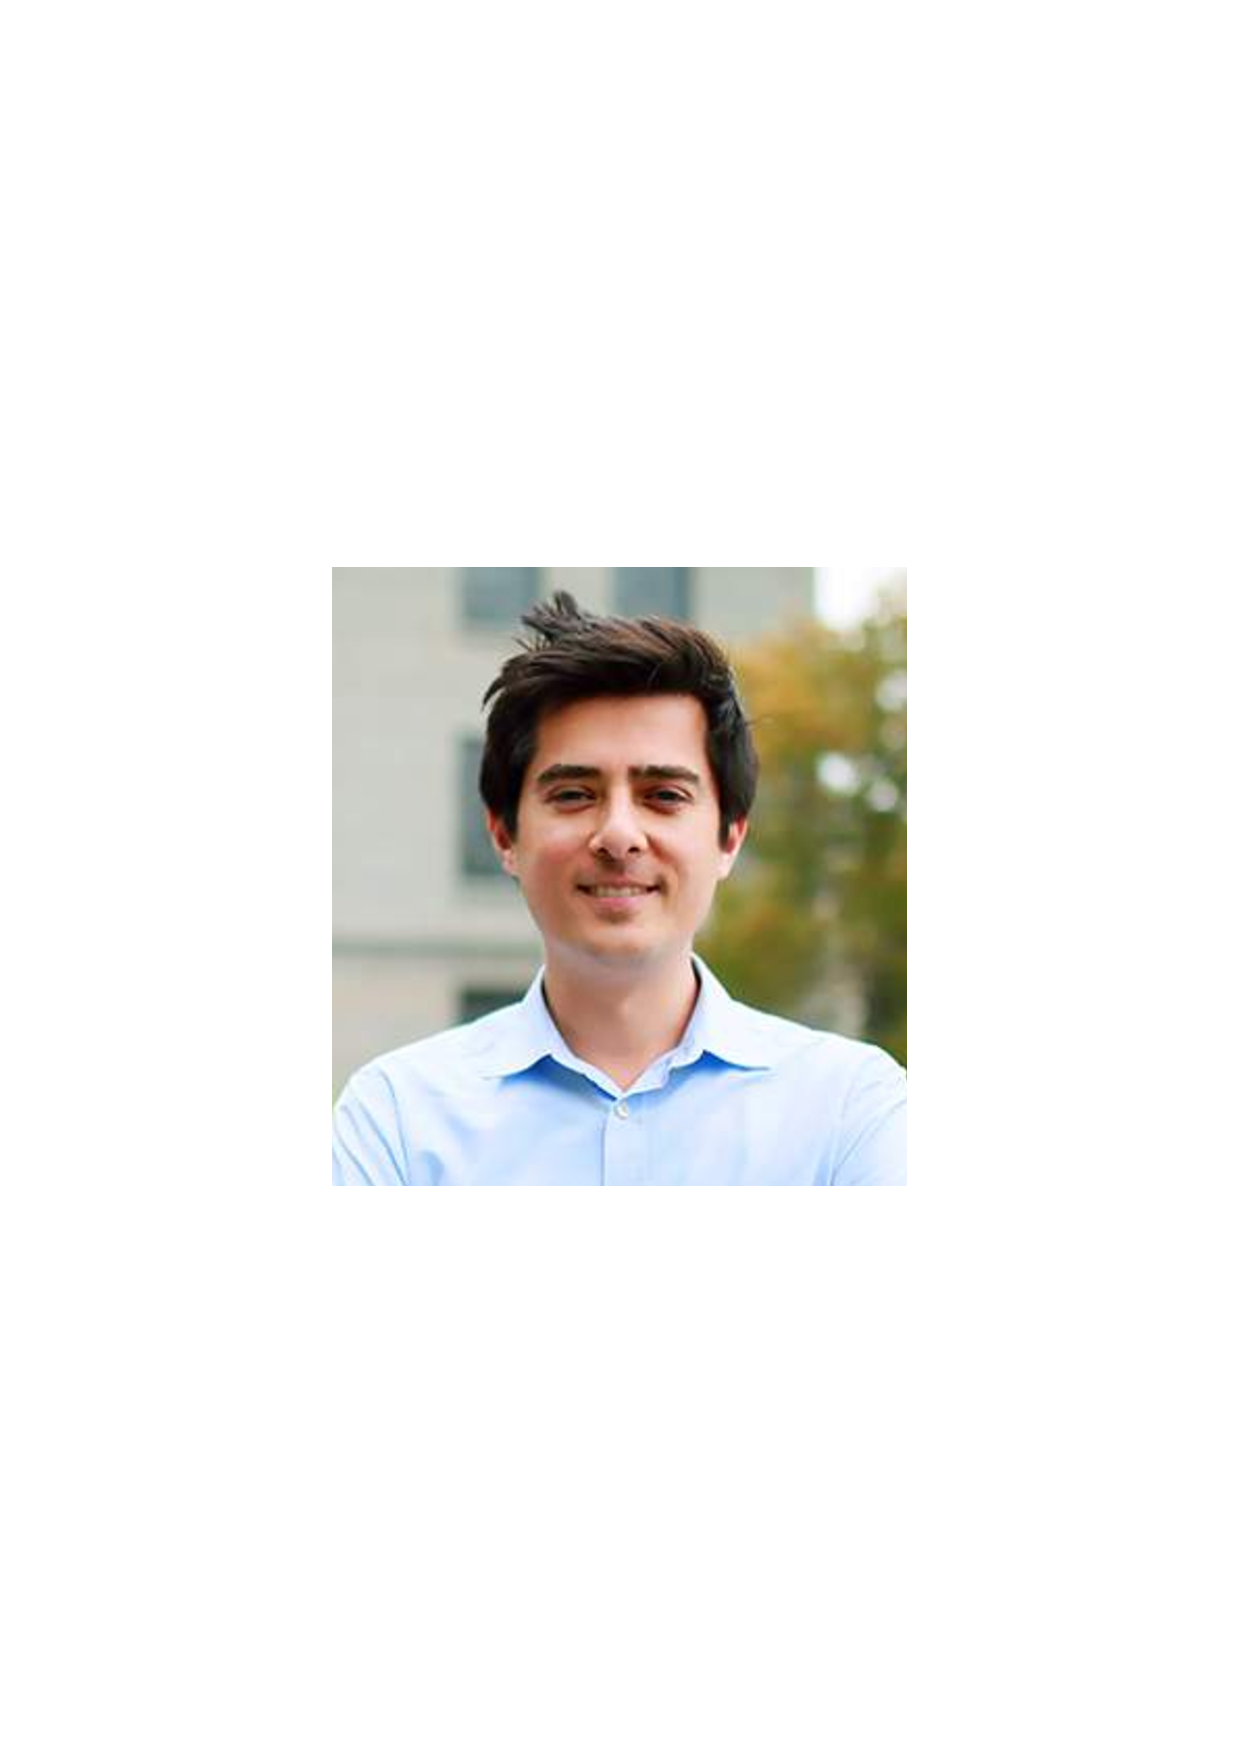
\includegraphics[width=0.47\textwidth]{photo_tim_byrnes}
\end{center}

Tim Byrnes....

\comment{Complete this section}

%
% Bill Munro
%

\begin{center}
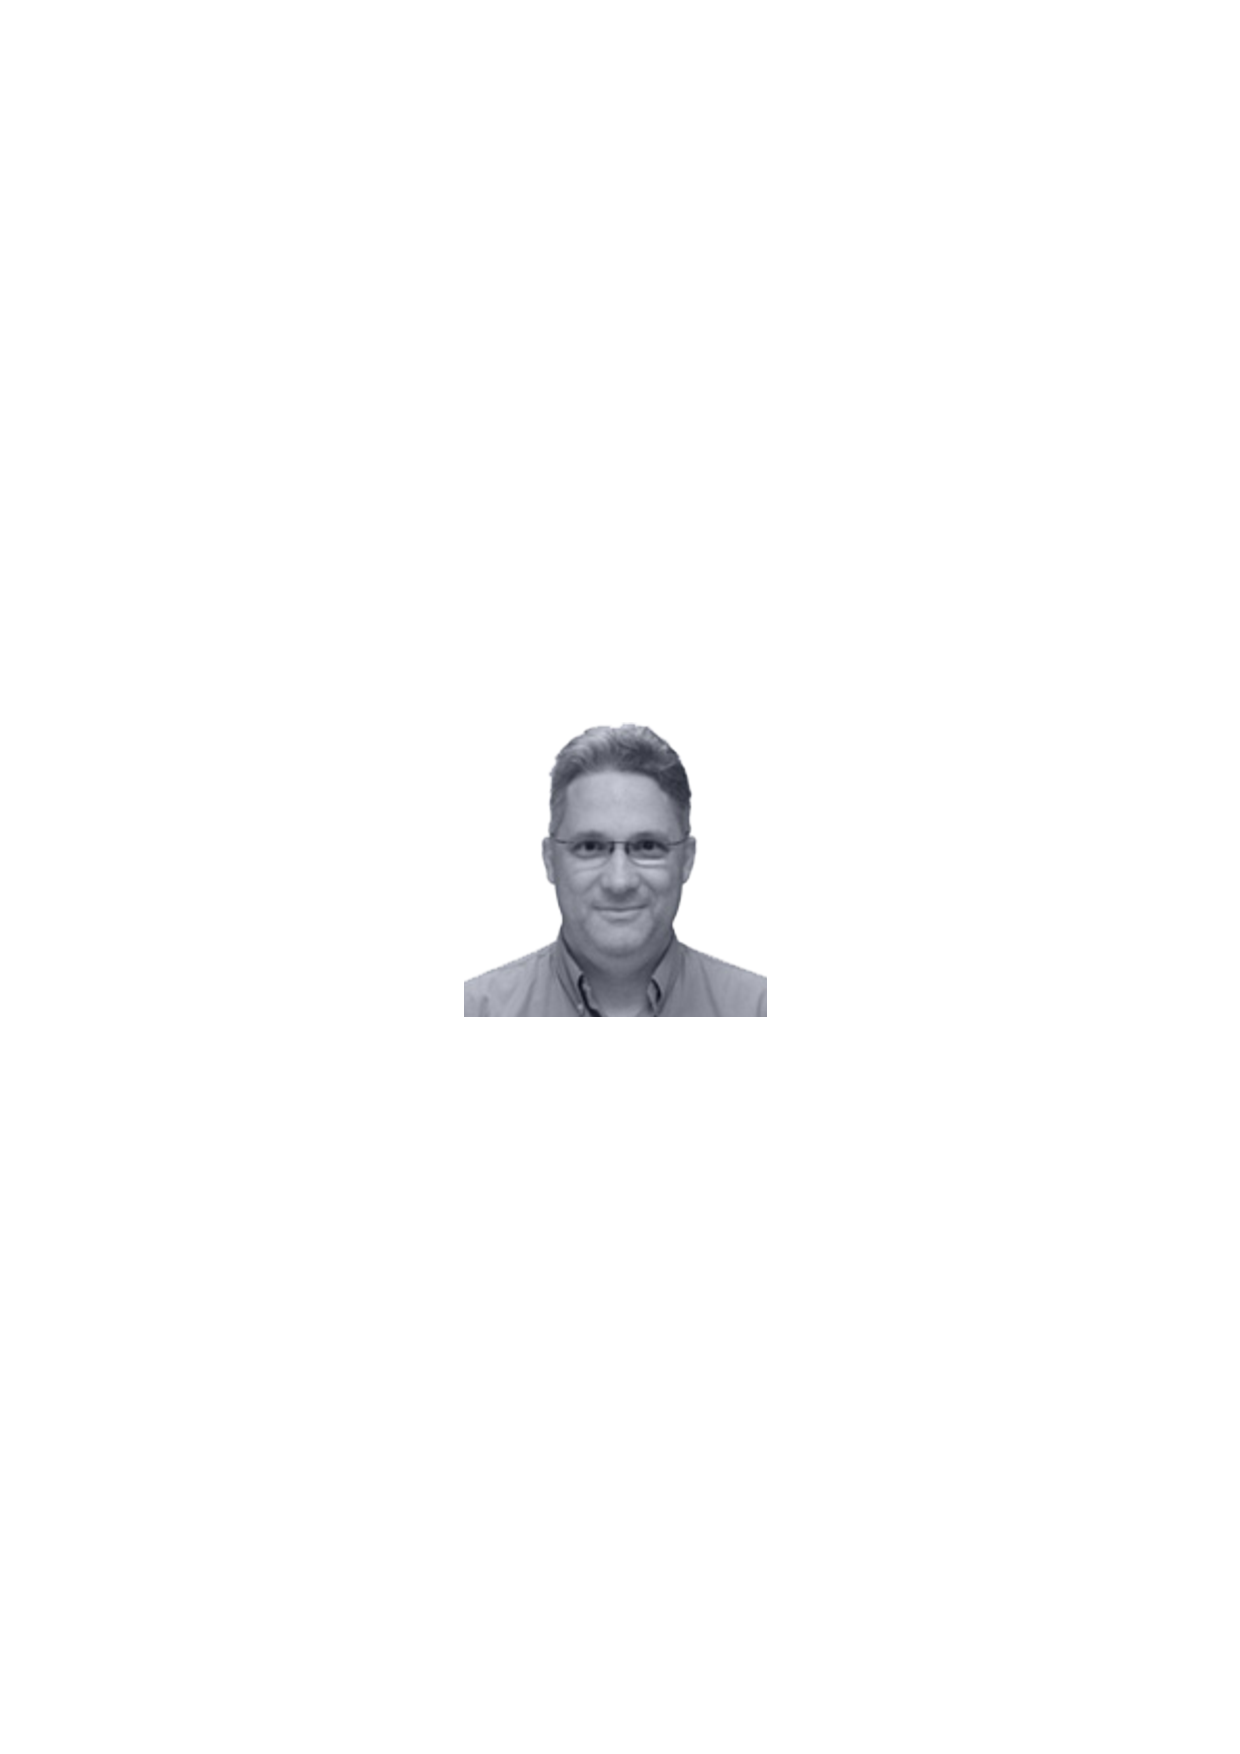
\includegraphics[width=0.47\textwidth]{photo_bill_munro}
\end{center}

Bill Munro obtained his PhD at the University of Waikato, and has since held numerous prestigious fellowships and positions. He is currently Senior Research Scientist and leader of the theoretical quantum physics research group at NTT Japan.

\comment{Complete this section}